%This texhead is for latex2e

% some new things
%
% \setlength{\epsfysize}{.8\textheight}
% \epsffile{mypic.eps}

\documentclass[12pt]{article}
\usepackage{fancyheadings}
\usepackage{hyperref}
\usepackage{graphicx}
\textwidth=6.2in
\textheight=8.5in
\parskip=.3cm
\oddsidemargin=.1in
\evensidemargin=.1in
\headheight=-.3in

\begin{document}
%\setkeys{Gin}{width=0.55\textwidth}


Mismatches in Dressman archive

The Excel spreadsheet at 
\url{
https://discovery.genome.duke.edu/express/resources/193/correctedplatinum_RMA.xls
}
has contents that we call RMA+SFR because arrays were preprocessed
by RMA and then by sparse factor regression.

The zip file at 
\url{https://discovery.genome.duke.edu/express/resources/1144/PlatinumJCO.zip}
has CEL files that have sample identifiers embedded in the filenames.
We apply RMA to these CEL files jointly.

Then we can see a display like this:

\setkeys{Gin}{width=0.65\textwidth}
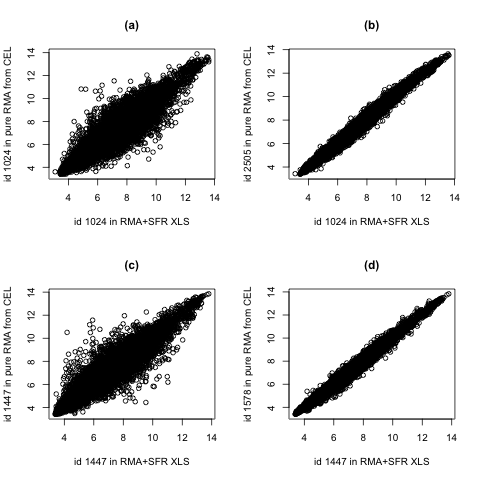
\includegraphics{corChk}


Panel (a) is the kind of scatterplot you see when two different
arrays are plotted against each other.  Panel (b) is the kind
of pattern you see when expression values on a given array
preprocessed in two different ways are plotted against each other.
(c) and (d) are a similar example.  Baggerly et al. originally
inferred that 87/119 samples in the RMA+SFR excel archive
needed to be relabeled on the basis of observations like these.

The full table of proposed relabelings can be seen in
pp 16-18 of
\url{http://bioinformatics.mdanderson.org/Supplements/ReproRsch-Ovary/ovca01.pdf}

\end{document}
